%%%%%%%%%%%%%%%%%%%%%%%%%%%%%%%%%%%%% 
%% LE2I beamer template
%% Guillaume Lemaitre, October 2014
%%%%%%%%%%%%%%%%%%%%%%%%%%%%%%%%%%%%% 

\documentclass{beamer}

\usepackage[utf8]{inputenc}
\usepackage[T1]{fontenc} 
\usetheme{le2i} 

%% The amssymb package provides various useful mathematical symbols
\usepackage{amssymb}
%% The amsthm package provides extended theorem environments
\usepackage{amsthm}
%% amsmath for math environment
\usepackage{amsmath}

\DeclareMathOperator*{\argmin}{arg\,min}
\DeclareMathOperator*{\argmax}{arg\,max}
\DeclareMathOperator*{\sign}{sign}

%% figure package
\usepackage{epsf,graphicx}
\usepackage{epstopdf}
\usepackage{subfigure}
\usepackage{transparent}
\usepackage{caption}
\captionsetup{font=scriptsize,labelfont=scriptsize,labelformat=empty}
\setbeamertemplate{caption}{\raggedright\insertcaption\par}
\usepackage{scalefnt,lmodern,booktabs}

%% In order to draw some graphs
\usepackage{tikz,xifthen}
\usepackage{tikz-qtree}
\usepackage{adjustbox}
\usetikzlibrary{decorations.pathmorphing}
\usetikzlibrary{fit}
\usetikzlibrary{backgrounds}
\usetikzlibrary{shapes,arrows,shadows}
\usetikzlibrary{calc,decorations.pathreplacing,decorations.markings,positioning}
\usetikzlibrary{snakes,decorations.text,shapes,patterns}
% \usepackage{scalefnt,lmodern,booktabs}

%% Package for cross and tick symbols
\usepackage{pifont}
\newcommand{\tick}{\color{green!60!black!80}\ding{51}}
\newcommand{\cross}{\color{red!60!black!80}\ding{55}}

\usepackage{enumitem}
\setitemize{label=\usebeamerfont*{itemize item}%
  \usebeamercolor[fg]{itemize item}
  \usebeamertemplate{itemize item}}

% \usepackage{apalike}
\usepackage[style=verbose,autocite=footnote,maxnames=10,babel=hyphen,hyperref=true,abbreviate=false,backend=biber,mcite]{biblatex}
\addbibresource{literature_review.bib}
\setbeamertemplate{footnote}{%
  \tiny%
  \parindent 1em\noindent%
  \raggedright
  \hbox to 1.8em{\hfil\insertfootnotemark}\insertfootnotetext\par%
}%
\setlength\footnotesep{0pt}

\title{\Large{Classification of SD-OCT Volumes with LBP: Application to DME Detection}}
\author{\scriptsize{G.~Lema\^itre, M.~Rastgoo, J.~Massich, S.~Shrinivasan, F.~M\'eriaudeau, and D.~Sidib\'e}}
\date{MICCAI-OMIA \\ 9\textsuperscript{th} Oct. 2015}

\institute{Universit\'e de Bourgogne \& Universitat de Girona} 

%% Uncomment if you want to avoid thousand of bullet inside the menu
% \usepackage{etoolbox}
% \makeatletter
% \patchcmd{\slideentry}{\advance\beamer@xpos by1\relax}{}{}{}
% \def\beamer@subsectionentry#1#2#3#4#5{\advance\beamer@xpos by1\relax}%
% \makeatother

\begin{document}

% Show the title page
\begin{frame}
  \titlepage
\end{frame}

% Show the table of contents
\begin{frame}
  \tableofcontents[sectionstyle=show,subsectionstyle=show,subsubsectionstyle=hide]
\end{frame}

\section{Introduction}

\subsection{Diabetic Macular Edema}

\begin{frame}
  \frametitle{Introduction}
  \framesubtitle{Diabetic Macular Edema (DME)}
  \begin{block}{DME}
    \begin{itemize}\footnotesize
    \item Breakdown of the blood-retinal barrier
    \item Leads to fluid leakage 
    \item Damage the photo-receptors 
    \end{itemize}
  \end{block}
  \begin{block}{SD-OCT}
    \begin{center}
      \only<1>{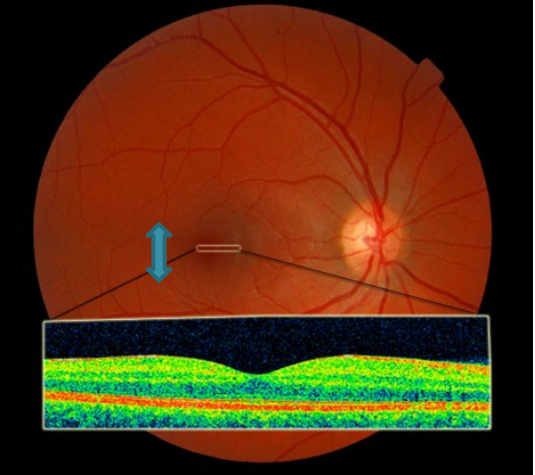
\includegraphics[scale=0.2]{images/OCT2.png}}
      \only<2>{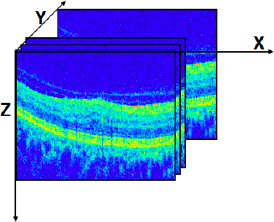
\includegraphics[scale=0.3]{images/volume.png}}
    \end{center}
  \end{block}
\end{frame}  

\begin{frame}
  \frametitle{Introduction}
  \framesubtitle{DME}
    \begin{block}{\footnotesize Cyst}
    \begin{center}
      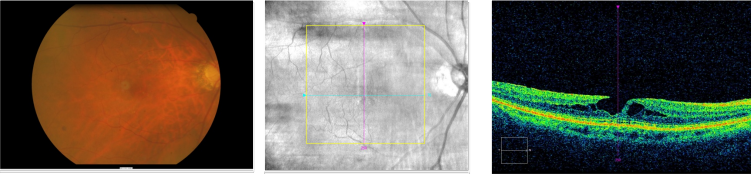
\includegraphics[scale=0.2]{images/Cyst_DME.png}
    \end{center}
  \end{block}
  \begin{block}{\footnotesize Hard Exudates}
    \begin{center}
      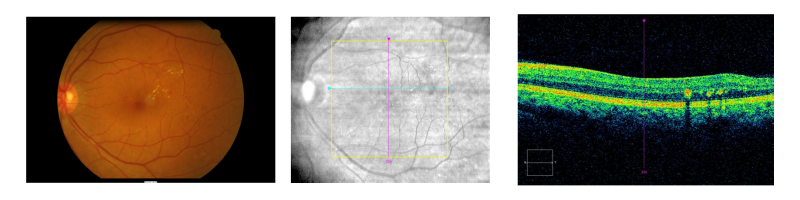
\includegraphics[scale=0.2]{images/HE_DME.png}
    \end{center}
  \end{block}
  \begin{block}{\footnotesize Sub Retinal Fluid}
    \begin{center}
      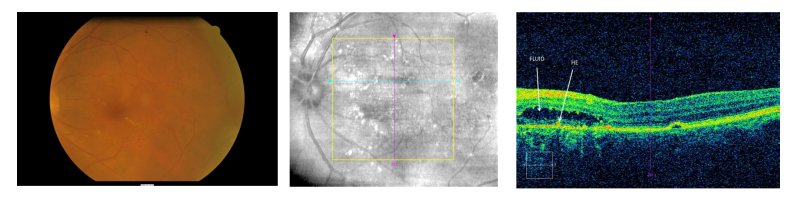
\includegraphics[scale=0.2]{images/SF_DME.png}
    \end{center}
  \end{block}
\end{frame}
% ---------------


\subsection{State-of-the-art}

\begin{frame}
  \frametitle{Introduction}
  \framesubtitle{State-of-the-art}
  \begin{block}{Srinivasan\,\textit{et al.}~\footnotemark }
    \begin{figure}
      \centering
      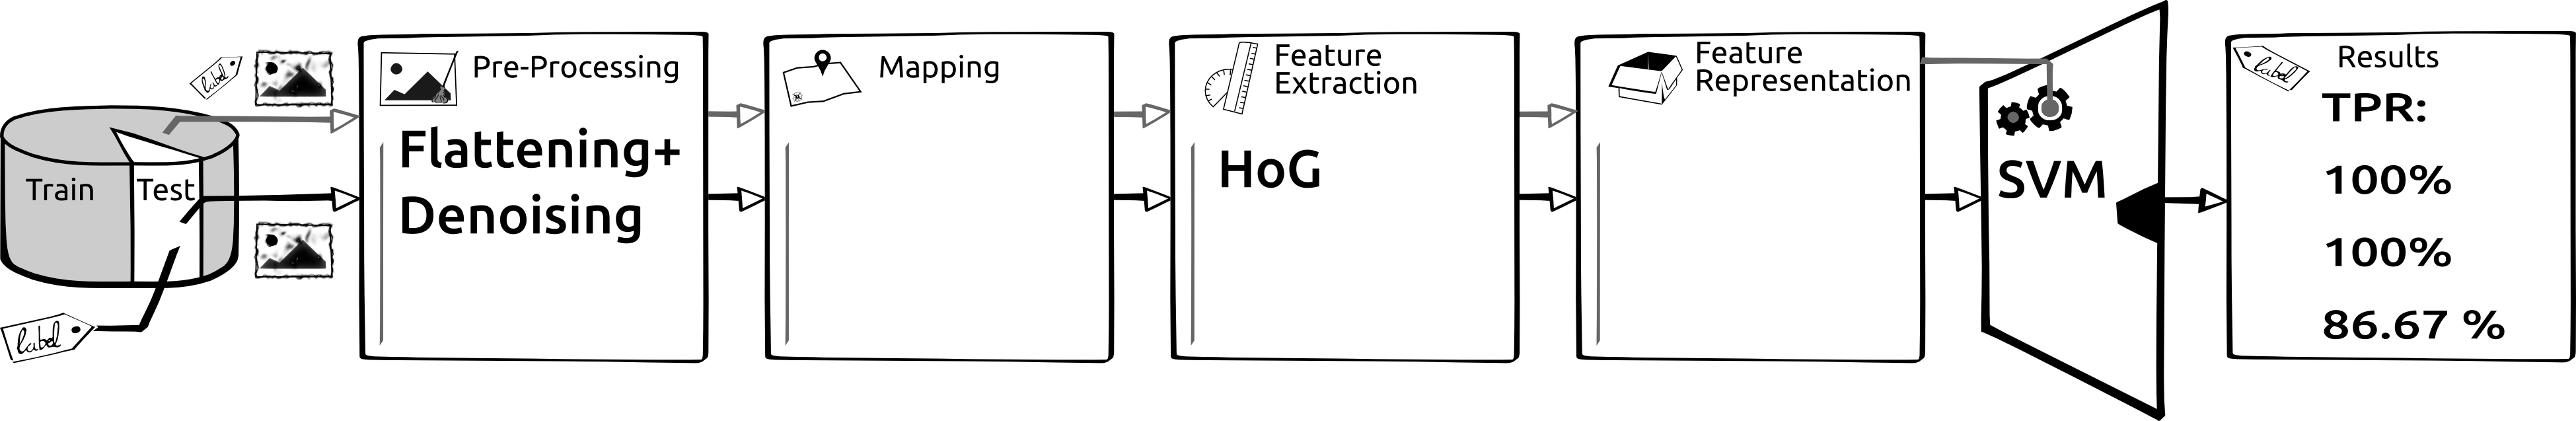
\includegraphics[width=1.\textwidth]{./images/srini.png}
      % \caption{Include an image}
    \end{figure}
  \end{block}
  \footcitetext{Srinivasan2014}
\end{frame}
% --------------
\begin{frame}
  \frametitle{State of the Art}
  \begin{block}{Venhuizen\,\textit{et al.}~\footnotemark}
    \begin{figure}
      \centering
      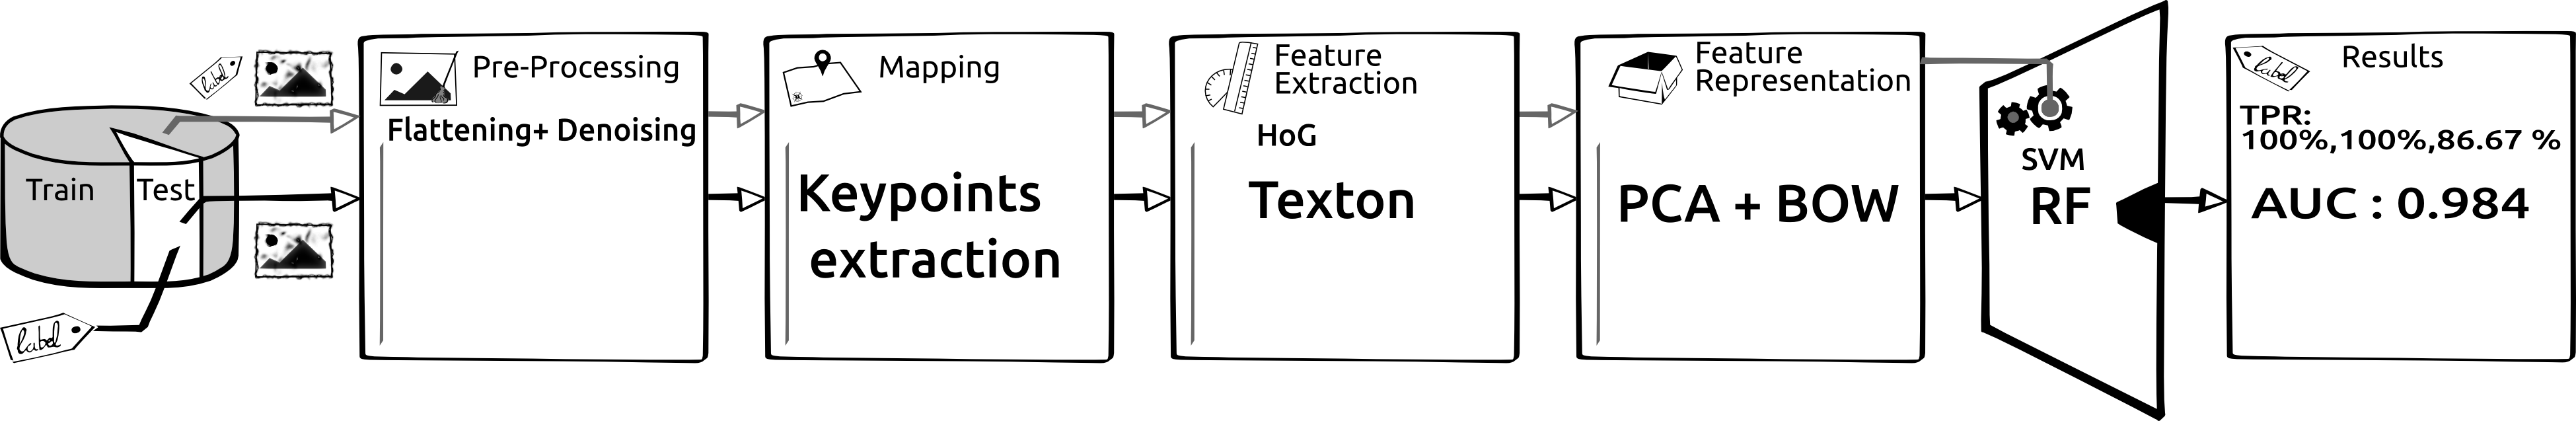
\includegraphics[width=1.\textwidth]{./images/ven.png}
      % \caption{Include an image}
    \end{figure}
  \end{block}
  \footcitetext{Venhuizen2015}
\end{frame}
% -------------
\begin{frame}
  \frametitle{State of the Art}
  \begin{block}{Liu\,\textit{et al.}~\footnotemark}
    \begin{figure}
      \centering
      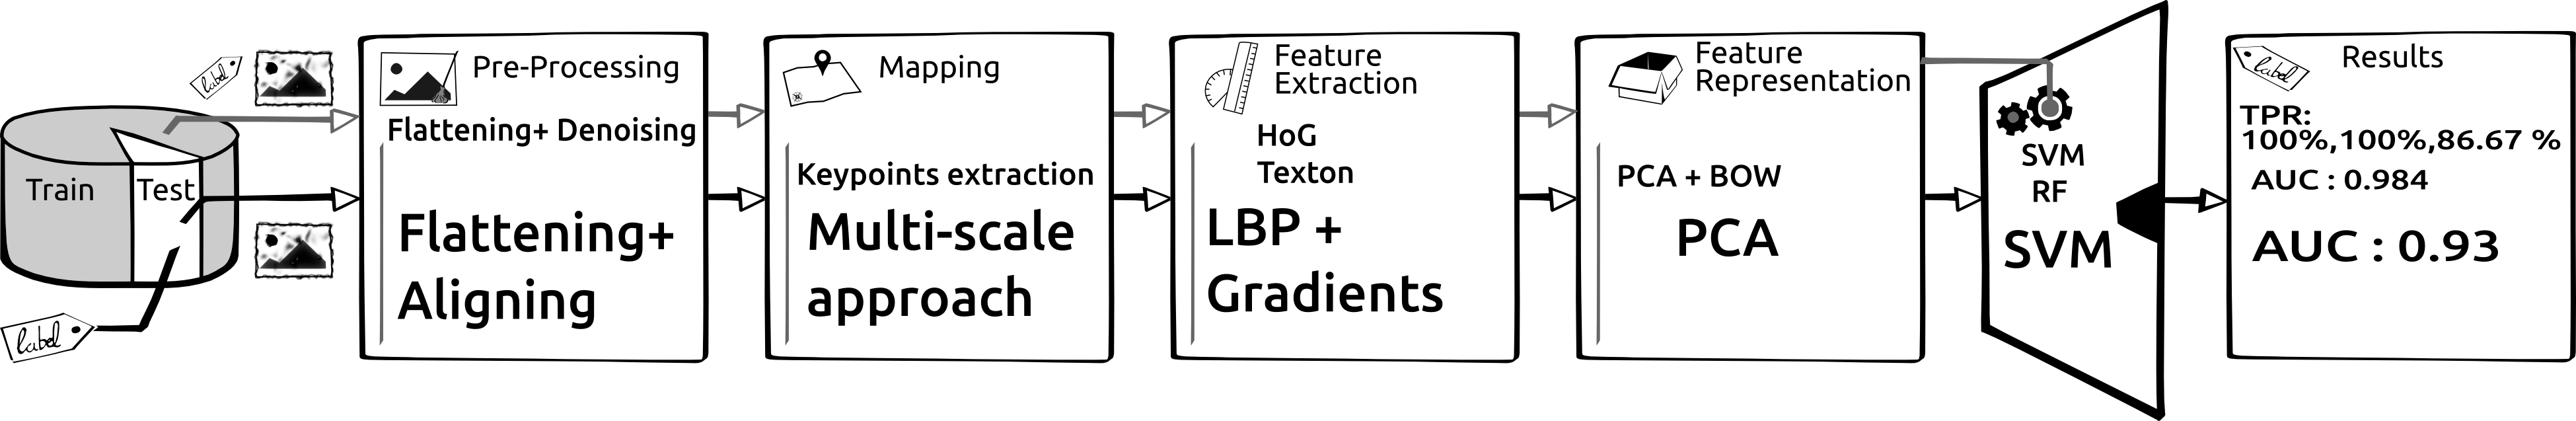
\includegraphics[width=1.\textwidth]{./images/liu.png}
      % \caption{Include an image}
    \end{figure}
  \end{block}
  \footcitetext{Liu2011}
\end{frame}

\section{DME detection}

\subsection{Framework}

\begin{frame}
  \frametitle{DME detection}
  \framesubtitle{Framework}
  \begin{block}{Overview}
    \begin{figure}
      \centering
      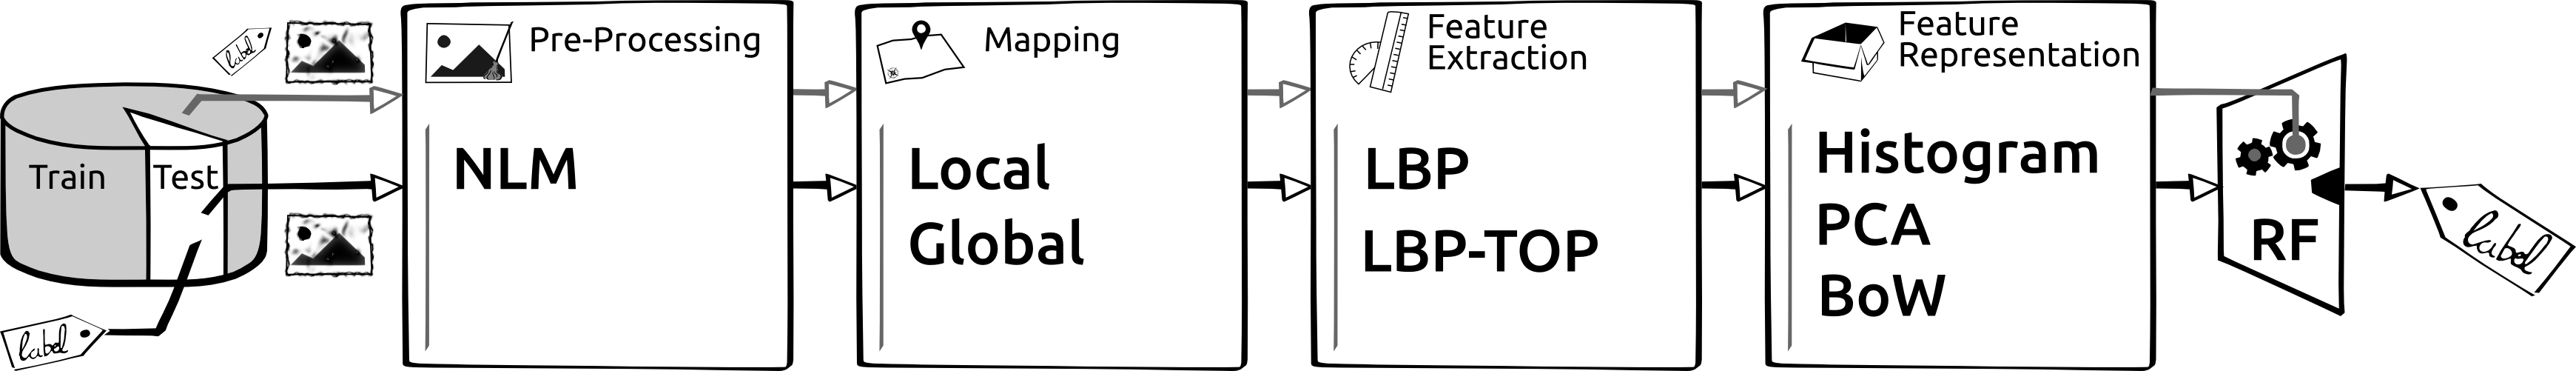
\includegraphics[width=1.\textwidth]{./images/ml.png}
      % \caption{Include an image}
    \end{figure}
  \end{block}
\end{frame}

\subsection{Image pre-processing}

\begin{frame}
  \frametitle{DME detection}
  \framesubtitle{Image pre-processing}
  \begin{figure}
    \centering
    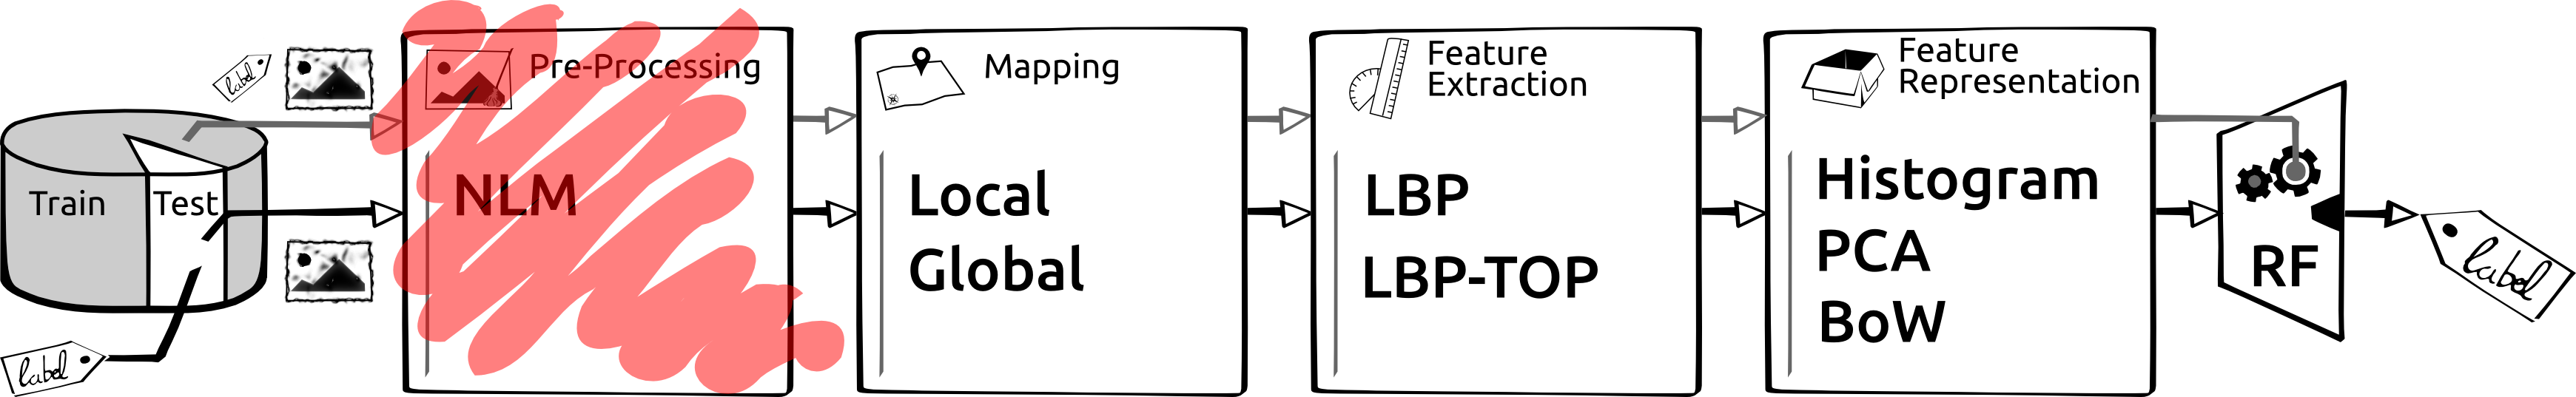
\includegraphics[width=.5\textwidth]{./images/ml-nlm.png}
    % \caption{Include an image}
  \end{figure}
  \begin{block}{Reference system}
    \begin{columns}
      \begin{column}{.3\linewidth}
        \begin{figure}
          \centering
          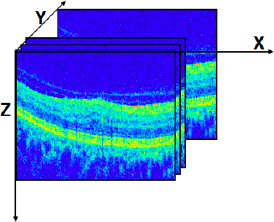
\includegraphics[width=.6\textwidth]{./images/volume.png}
          % \caption{Include an image}
        \end{figure}
      \end{column}
      \begin{column}{.6\linewidth}
        \begin{itemize}[leftmargin=*]\footnotesize
        \item OCT images corrupted with speckle noise
        \item Denoising for each B-scan ($x-z$ slice)
        \item \textbf{Non-Local Means}~\footnotemark
        \end{itemize}
      \end{column}
    \end{columns}
  \end{block}
  \footcitetext{Coupe2009}
\end{frame}


\begin{frame}
  \frametitle{DME detection}
  \framesubtitle{Image pre-processing}
  \begin{figure}
    \centering
    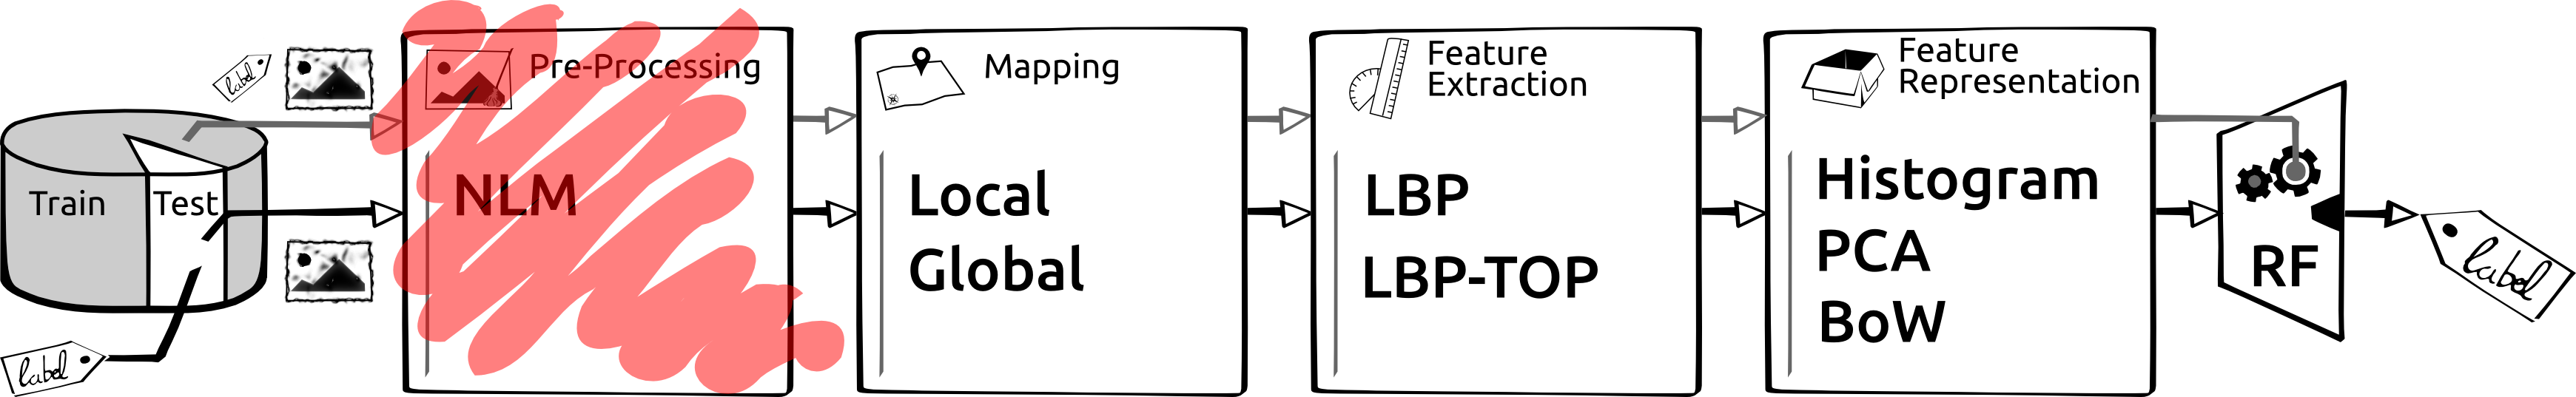
\includegraphics[width=.5\textwidth]{./images/ml-nlm.png}
    % \caption{Include an image}
  \end{figure}
  \begin{block}{Qualitative results}
    \begin{columns}
      \begin{column}{.5\linewidth}
        \begin{figure}
          \centering
          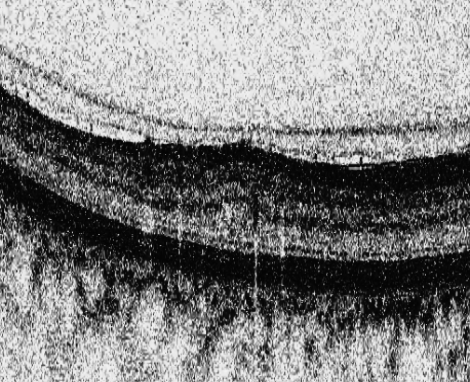
\includegraphics[width=.4\textwidth]{./images/raw_crop_grey.png}
          \caption{Raw image}
        \end{figure}
      \end{column}
      \begin{column}{.5\linewidth}
        \begin{figure}
          \centering
          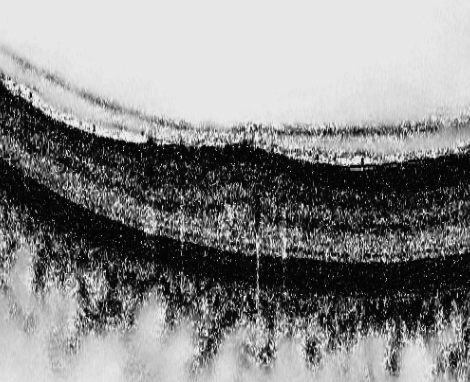
\includegraphics[width=.4\textwidth]{./images/nlm_crop_grey.png}
          \caption{NLM denoising}
        \end{figure}
      \end{column}
    \end{columns}
  \end{block}
\end{frame}

\subsection{Mapping}

\begin{frame}
  \frametitle{DME Detection}
  \framesubtitle{Mapping}
  \begin{figure}
    \centering
    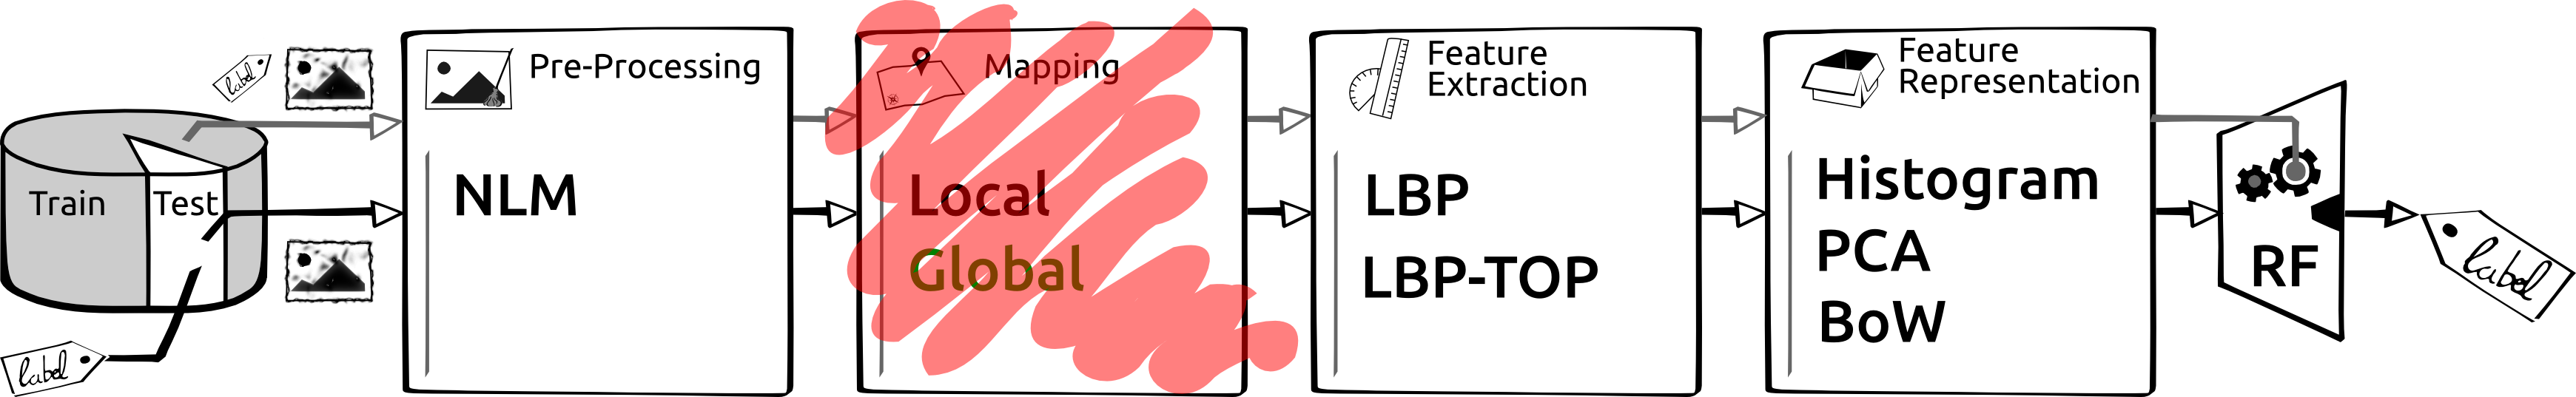
\includegraphics[width=.5\textwidth]{./images/ml-map2.png}
    % \caption{Include an image}
  \end{figure}
  \begin{block}{Global mapping}
    \begin{columns}
      \begin{column}{.5\linewidth}
        \begin{figure}
          \centering
          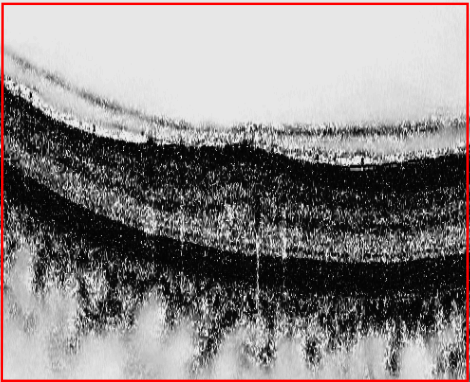
\includegraphics[width=.3\textwidth]{./images/global-2d.png}
          \caption{2D}
        \end{figure}
      \end{column}
      \begin{column}{.5\linewidth}
        \begin{figure}
          \centering
          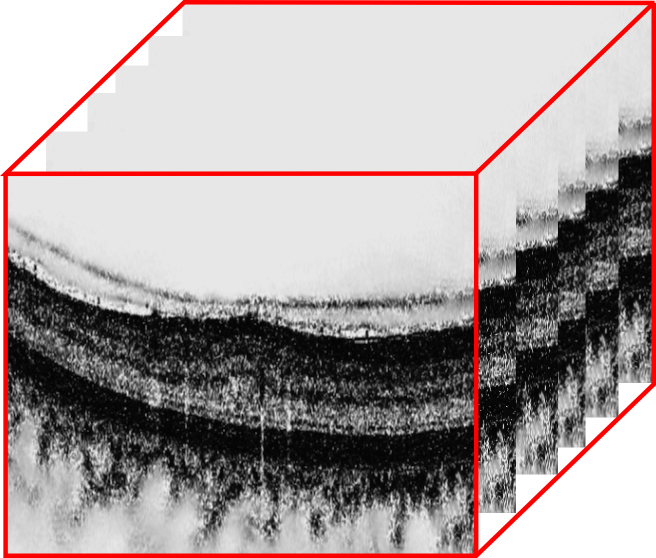
\includegraphics[width=.3\textwidth]{./images/global-3d.png}
          \caption{3D}
        \end{figure}
      \end{column}
    \end{columns}
  \end{block}
\end{frame}


\begin{frame}
  \frametitle{DME Detection}
  \framesubtitle{Mapping}
  \begin{figure}
    \centering
    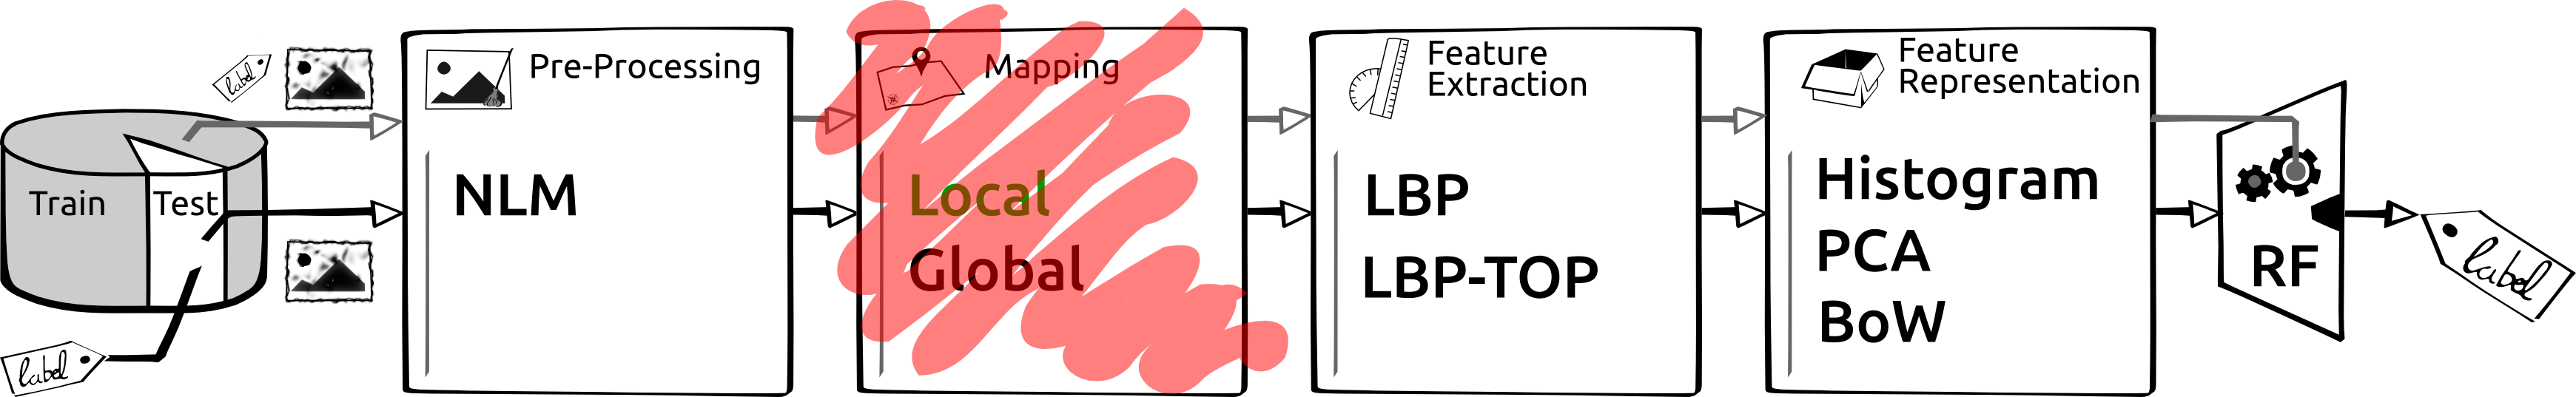
\includegraphics[width=.5\textwidth]{./images/ml-map1.png}
    % \caption{Include an image}
  \end{figure}
  \begin{block}{Local mapping}
    \begin{columns}
      \begin{column}{.5\linewidth}
        \begin{figure}
          \centering
          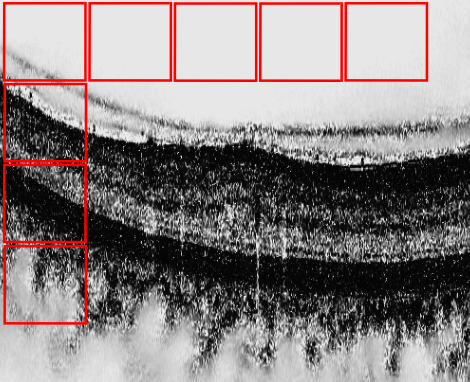
\includegraphics[width=.3\textwidth]{./images/local-2d.png}
          \caption{2D}
        \end{figure}
      \end{column}
      \begin{column}{.5\linewidth}
        \begin{figure}
          \centering
          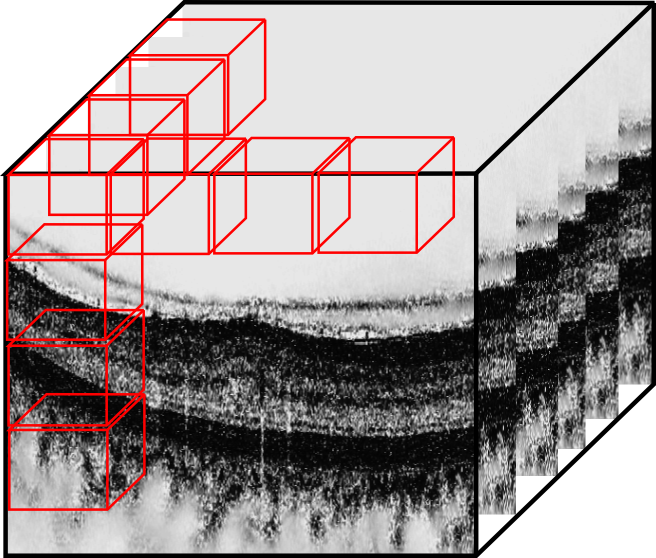
\includegraphics[width=.3\textwidth]{./images/local-3d.png}
          \caption{3D}
        \end{figure}
      \end{column}
    \end{columns}
  \end{block}
\end{frame}

\subsection{Local Binary Pattern}

\begin{frame}
  \frametitle{DME Detection}
  \framesubtitle{Local Binary Pattern (LBP)}
  \begin{figure}
    \centering
    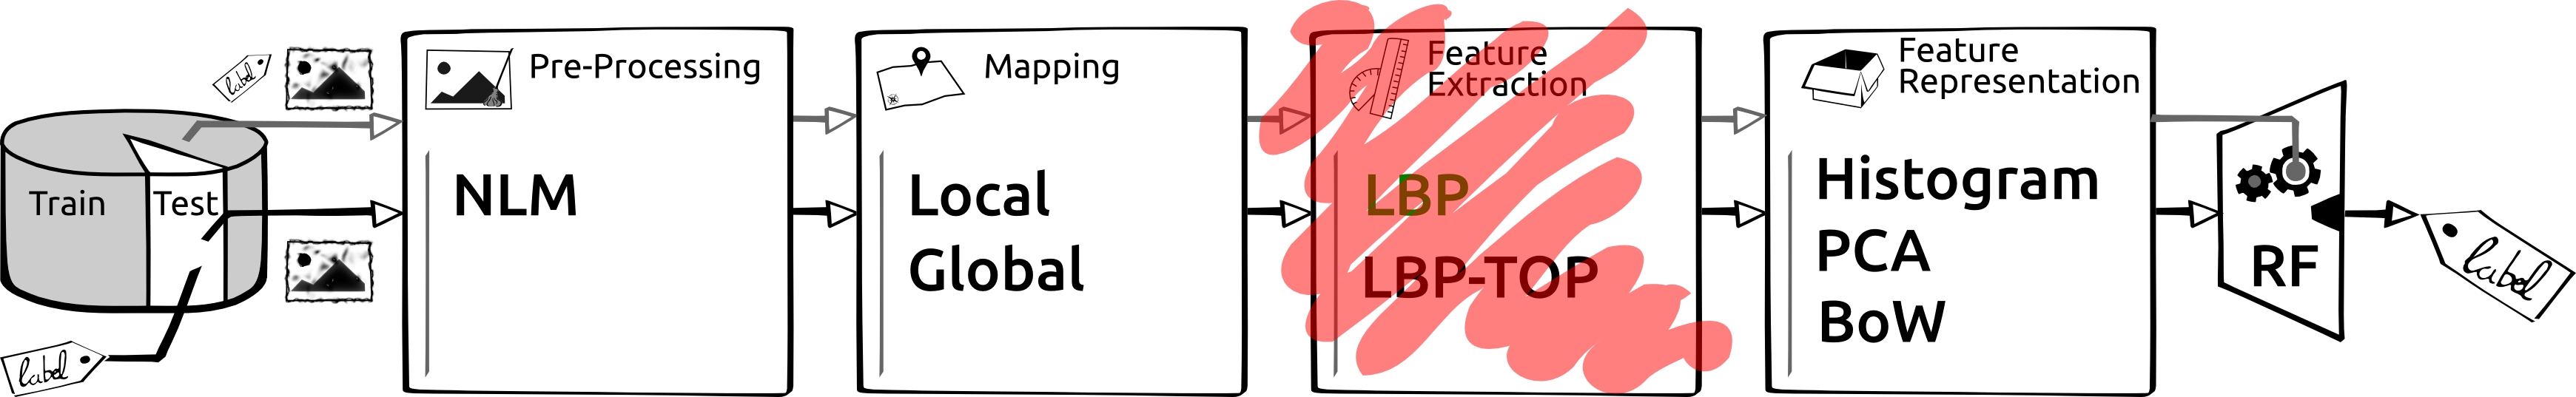
\includegraphics[width=.5\textwidth]{./images/ml-fe1.png}
    % \caption{Include an image}
  \end{figure}
  \begin{block}{LBP}
    \begin{columns}
      \begin{column}{.4\linewidth}
        \begin{figure}
          \centering
          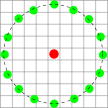
\includegraphics[width=.4\textwidth]{./images/lbp.png}
          % \caption{Raw image}
        \end{figure}
      \end{column}
      \begin{column}{.6\linewidth}
        {\tiny
          \begin{align*}\hspace*{-1cm}
            LBP_{P,R} = \sum_{p=0}^{P-1}s(g_{p} - g_{c})2^{p} \ ,~ s(\cdot) = \begin{cases}                                  
              1  & \ \text{if } (g_{p} - g_{c}) \geq 0\\                                                                         
              0  & \ \text{otherwise}\\                                                                                          
            \end{cases} \ ,                                                                                                        
          \end{align*}}%
        \begin{itemize}[leftmargin=*]\footnotesize
        \item Select uniform and rotation invariant
        \end{itemize}
      \end{column}
    \end{columns}
  \end{block}
\end{frame}

\begin{frame}
  \frametitle{DME Detection}
  \framesubtitle{LBP}
  \begin{figure}
    \centering
    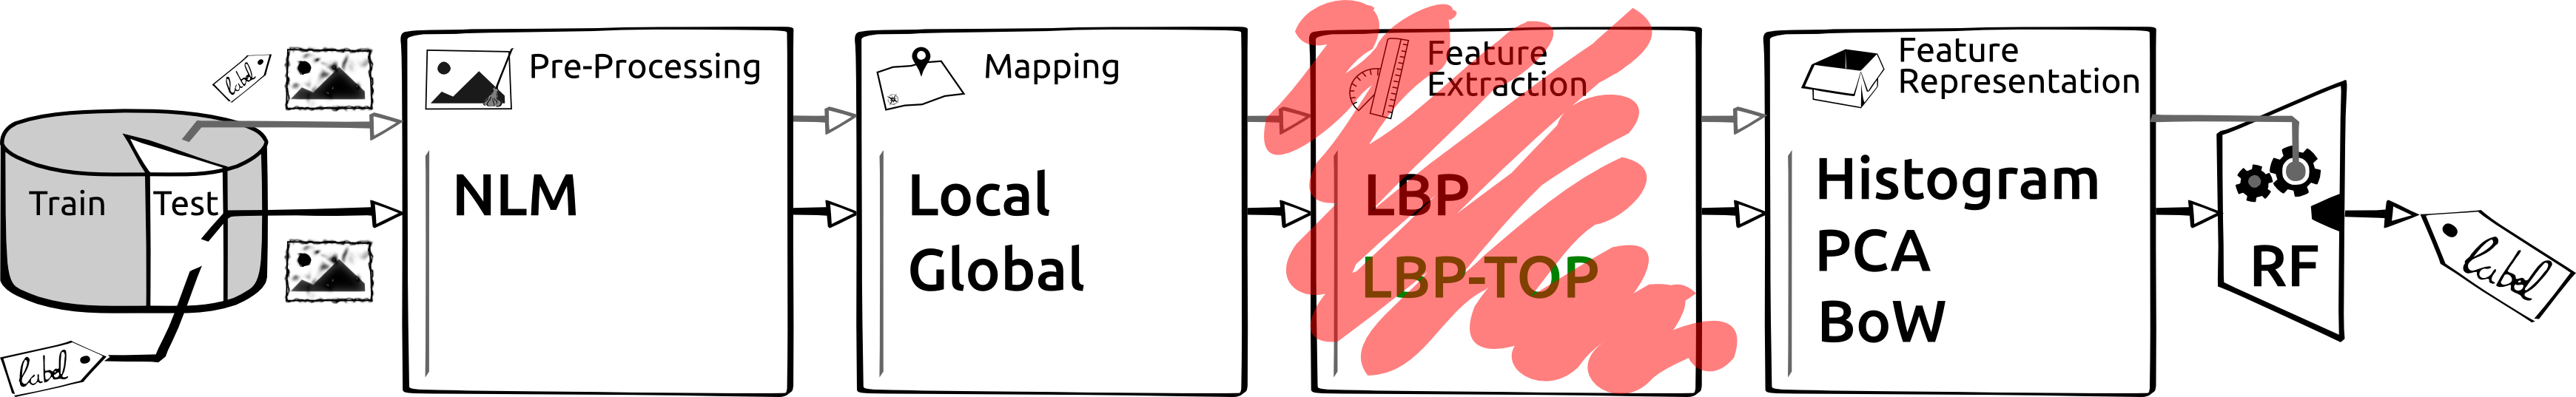
\includegraphics[width=.5\textwidth]{./images/ml-fe2.png}
    % \caption{Include an image}
  \end{figure}
  \begin{block}{LBP-Three Orthogonal Plane (TOP)}
    \begin{figure}
      \centering
      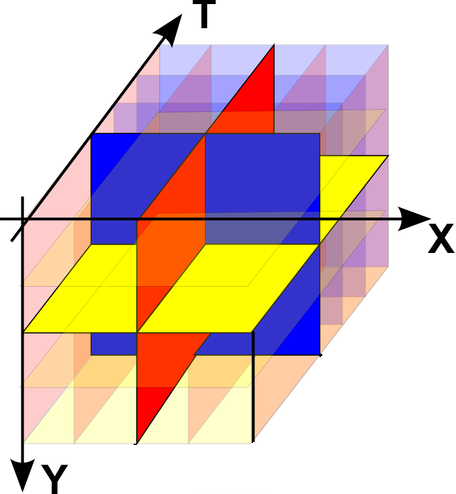
\includegraphics[width=.2\textwidth]{./images/lbp_top.png}
      % \caption{Raw image}
    \end{figure}
  \end{block}
\end{frame}

\subsection{Feature representation}

\begin{frame}
  \frametitle{DME Detection}
  \framesubtitle{Feature representation}
    \begin{figure}
    \centering
    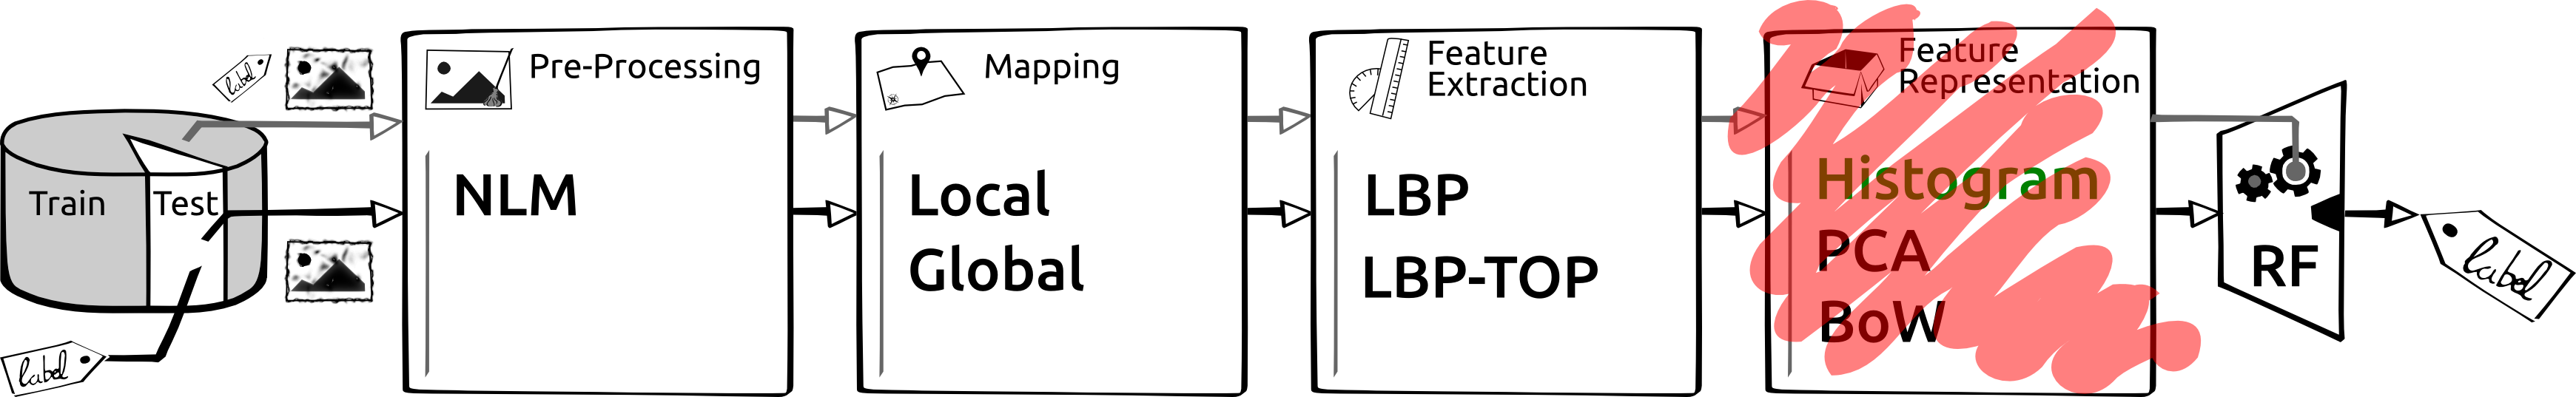
\includegraphics[width=.5\textwidth]{./images/ml-r1.png}
    % \caption{Include an image}
  \end{figure}
  \begin{block}{Low-level representation}\footnotesize
    \begin{center}
      $\rightarrow$ Compute the histogram of the LBP codes
    \end{center}
    \vspace{-.6cm}
    \begin{columns}
      \begin{column}{.5\linewidth}
        \begin{figure}
          \centering
          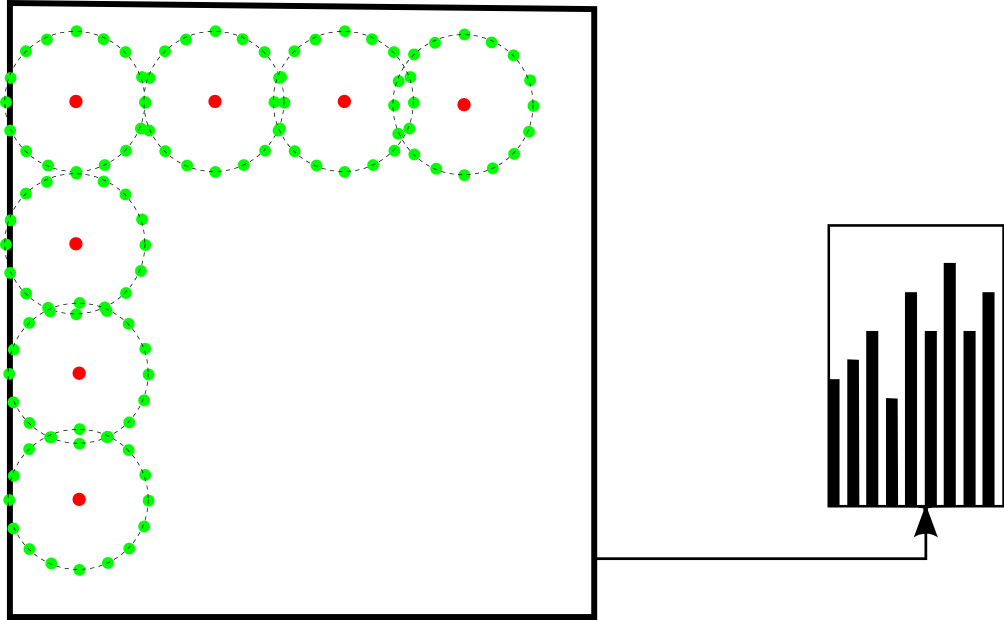
\includegraphics[width=.4\textwidth]{./images/lbp-hist.png}
          \caption{LBP histogram}
        \end{figure}
      \end{column}
      \begin{column}{.5\linewidth}
        \begin{figure}
          \centering
          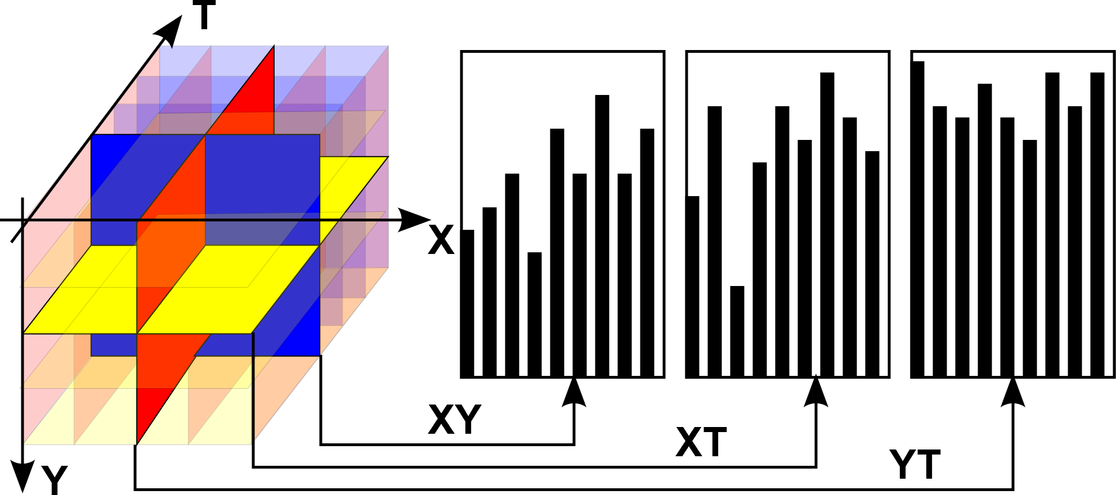
\includegraphics[width=.5\textwidth]{./images/LBPTOP_fig.png}
          \caption{LBP-TOP histogram}
        \end{figure}
      \end{column}
    \end{columns}
  \end{block}
\end{frame}


\begin{frame}
  \frametitle{DME Detection}
  \framesubtitle{Feature representation}
  \begin{figure}
    \centering
    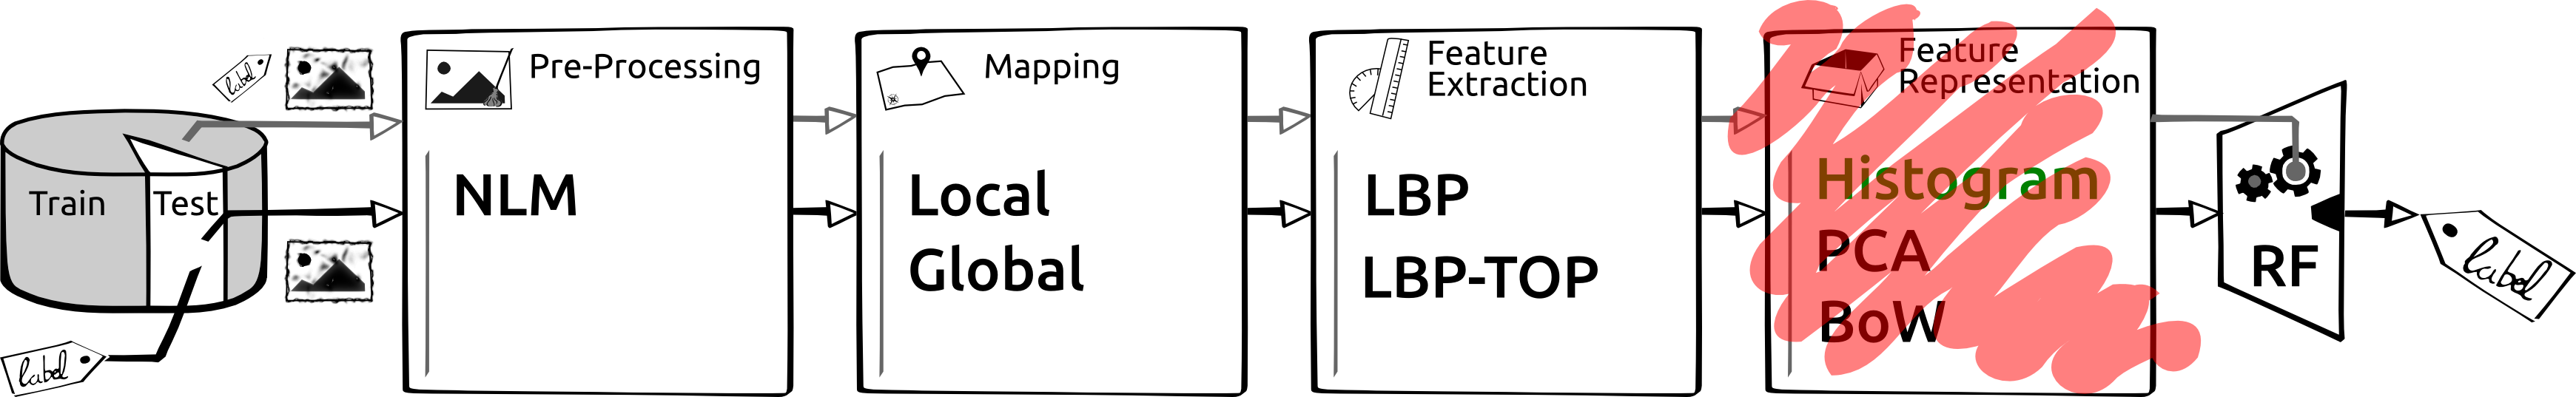
\includegraphics[width=.5\textwidth]{./images/ml-r1.png}
    % \caption{Include an image}
  \end{figure}
  \begin{block}{Global \textit{versus} local mapping}
    \begin{columns}
      \begin{column}{.5\linewidth}
        \begin{itemize}\footnotesize
        \item 1 LBP histogram per \emph{B-scan} later concatenated
        \item 1 LBP-TOP histogram per \emph{volume}
        \end{itemize}
      \end{column}
      \begin{column}{.5\linewidth}
        \begin{itemize}\footnotesize
        \item 1 LBP histogram per \emph{window} later concatenated
        \item 1 LBP-TOP histogram per \emph{sub-volume} later concatenated
        \end{itemize}
      \end{column}
    \end{columns}
  \end{block}
\end{frame}

\begin{frame}
  \frametitle{DME Detection}
  \framesubtitle{Feature representation}
  \begin{figure}
    \centering
    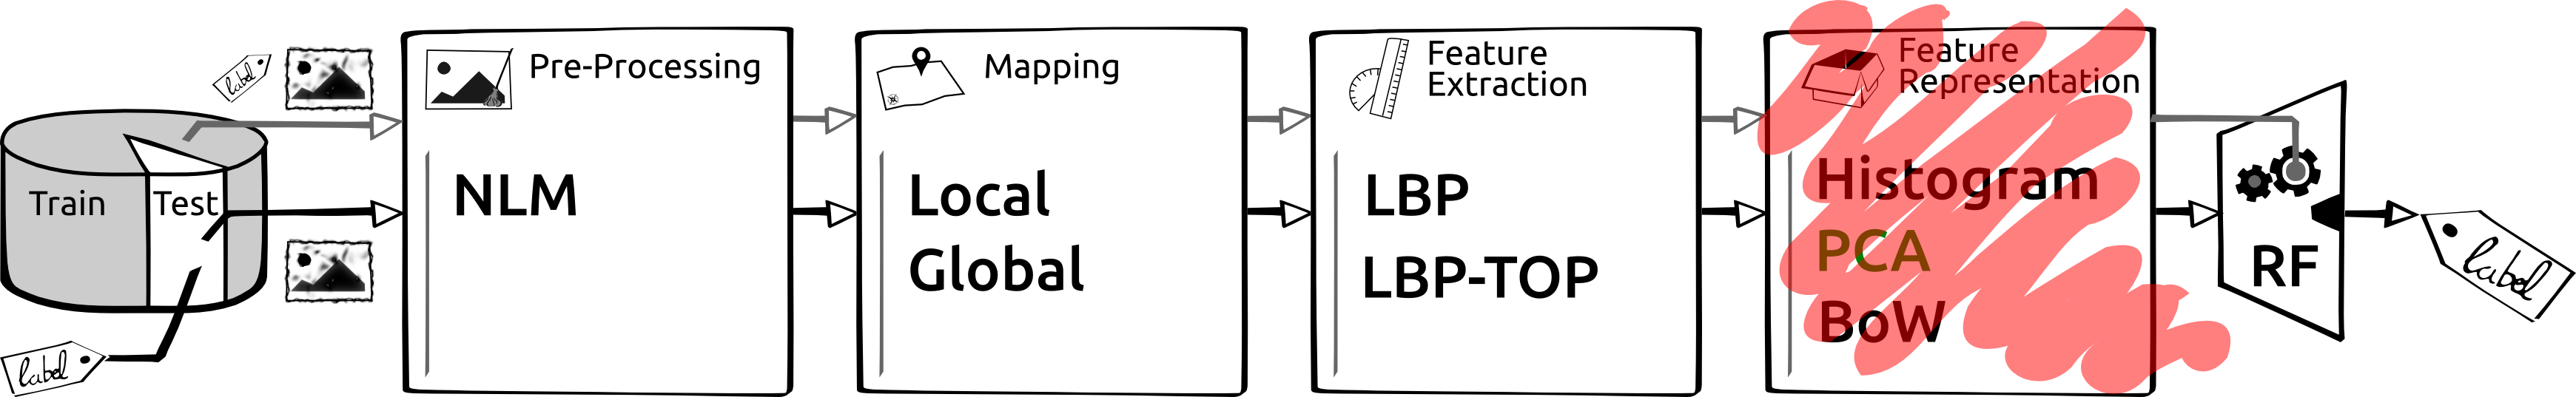
\includegraphics[width=.5\textwidth]{./images/ml-r2.png}
    % \caption{Include an image}
  \end{figure}
  \begin{block}{High-level representation --- PCA}
    \begin{itemize}\footnotesize
    \item Reduce the number of feature dimensions by finding a space where the data variance is maximized
    \end{itemize}
  \end{block}
\end{frame}

\begin{frame}
  \frametitle{DME Detection}
  \framesubtitle{Feature representation}
  \begin{figure}
    \centering
    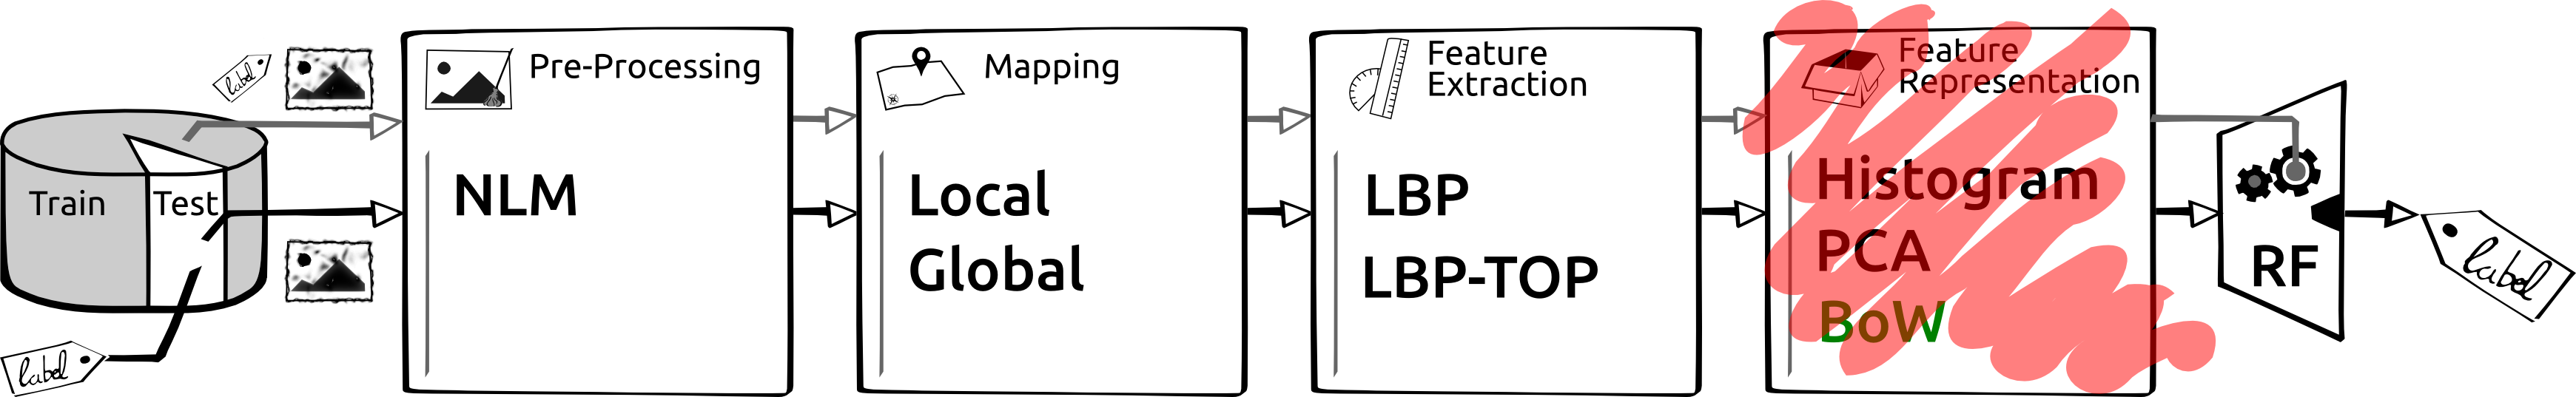
\includegraphics[width=.5\textwidth]{./images/ml-r3.png}
    % \caption{Include an image}
  \end{figure}
  \begin{block}{High-level representation --- BoW}
    \begin{itemize}\footnotesize
    \item Reduce the complexity of the feature space by clustering samples together
        \begin{figure}
          \centering
          \only<1>{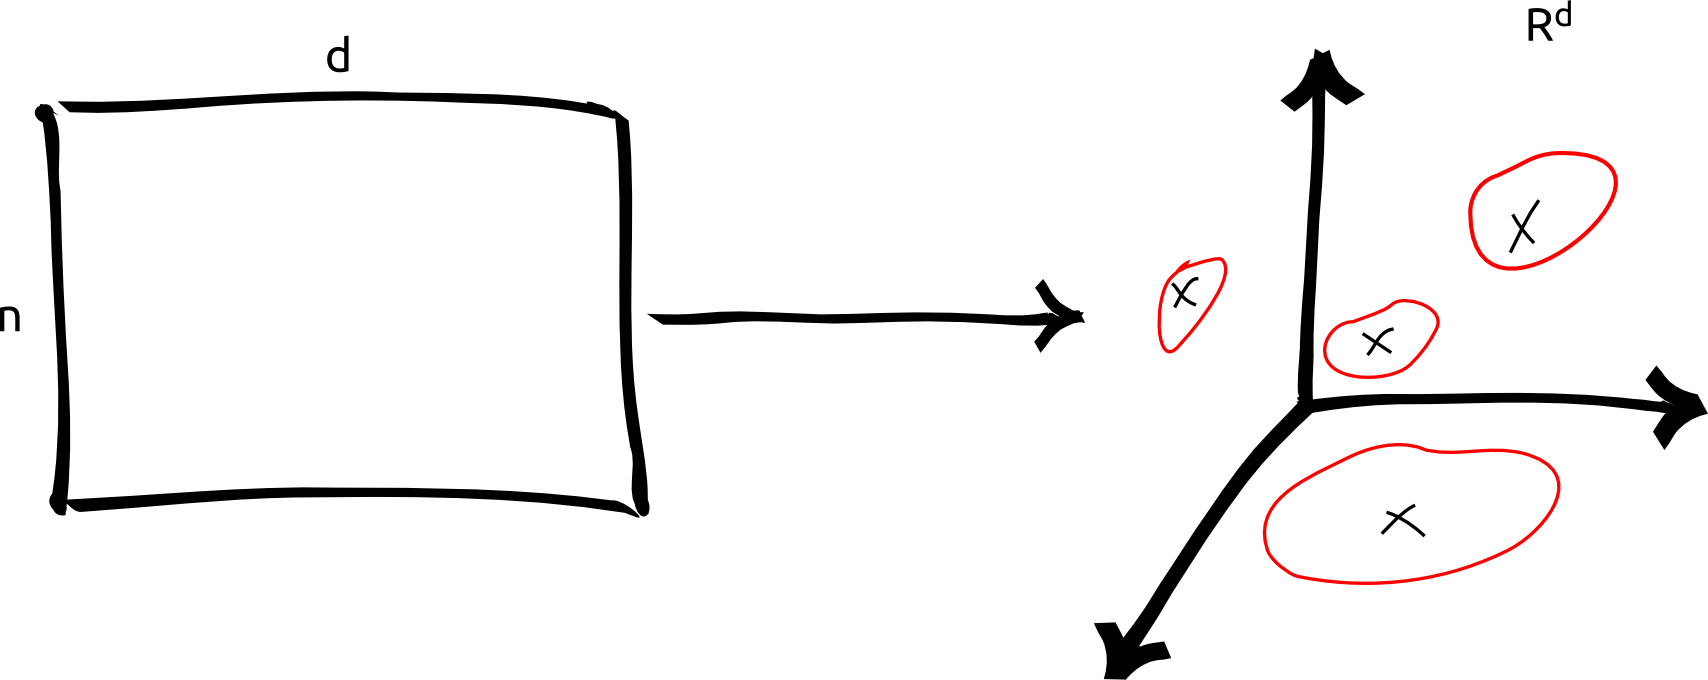
\includegraphics[width=.5\textwidth]{./images/bow-1.png}}
          \only<2>{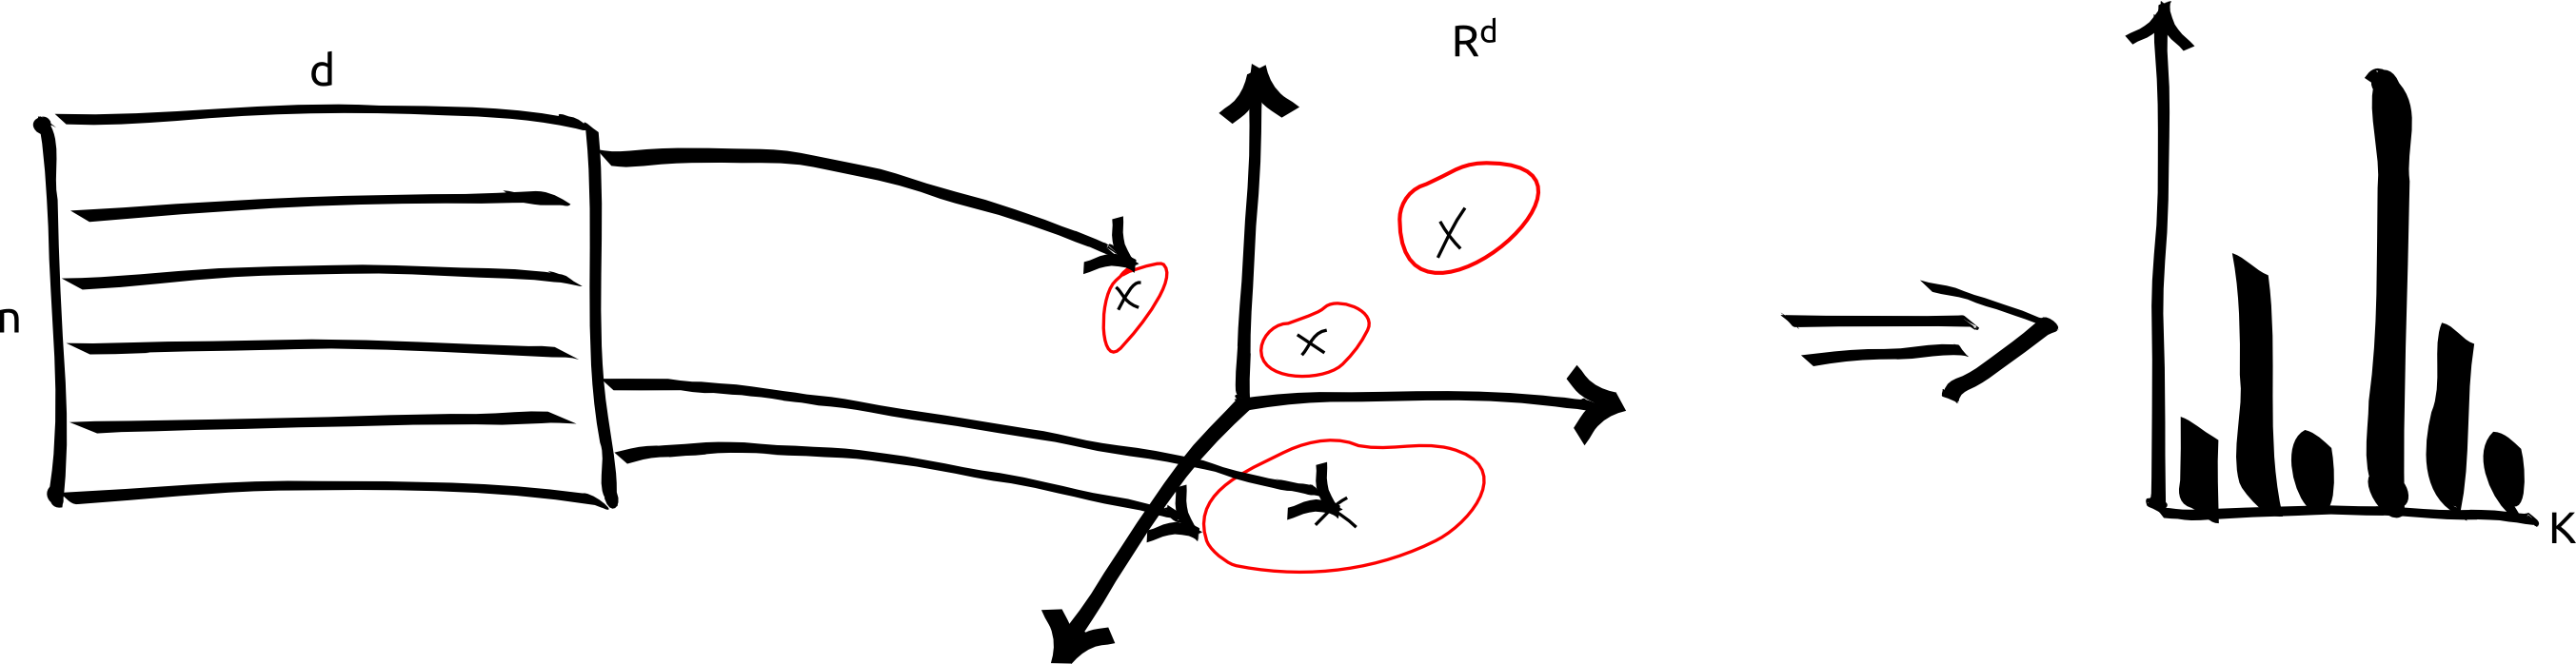
\includegraphics[width=.5\textwidth]{./images/bow-2.png}}
          % \caption{Include an image}
        \end{figure}
    \item<1-> A codebook is learnt through k-means
    \item<2-> Each sample is affected to a specific cluster/word (i.e., hard-voting)
    \item<2-> Histogram by calculating the frequency of occurrences of each word 
    \end{itemize}
  \end{block}
\end{frame}

\section{Experiments}

\subsection{Datasets}

\begin{frame}
  \frametitle{Experiments}
  \framesubtitle{Datasets}
  \begin{block}{SERI dataset}\footnotesize
    \begin{itemize}
    \item 32 SD-OCT images with 16 DME cases and 16 healthy cases
    \item Each volume has 128 B-scans with a resolution of $512 \times 1024$ pixels
    \end{itemize}
  \end{block}
  \begin{block}{Duke dataset}
    \begin{itemize}\footnotesize
    \item 30 SD-OCT images with 15 DME cases and 15 healthy cases
    \item Volumes were denoised and cropped with different sizes
    \end{itemize}
  \end{block}
\end{frame}

\begin{frame}
  \frametitle{Experiments}
  \framesubtitle{Parameters}
  \begin{block}{\footnotesize Local mapping}\footnotesize
    \begin{itemize}
    \item Window of $7 \times 7$ pixels and Sub-volume of $7 \times 7 \times 7$ pixels
    \end{itemize}
  \end{block}
  \begin{block}{\footnotesize LBP generation}\footnotesize
    \begin{itemize}
    \item Radius of 1, 2, and 3 pixels
    \item 8, 16, and 24 neighbours
    \end{itemize}
  \end{block}
  \begin{block}{\footnotesize High-level representation}\footnotesize
    \begin{itemize}
    \item PCA keeping eigenvectors with the 99 \% cumulative eigenvalues
    \item Codebook of 32 words
    \end{itemize}
  \end{block}
  \begin{block}{\footnotesize Classification}\footnotesize
    \begin{itemize}
    \item Leave-One-Patient-Out cross-validation 
    \item Random Forest classifier with 100 trees
    \end{itemize}
  \end{block}
\end{frame}

\begin{frame}
\frametitle{Experiments}
\begin{block}{Experiment~\#1}
\begin{itemize}\footnotesize
\item SERI dataset 
\item 2D B-scan and 3D volumes, local and global mapping
\item Low and high feature representation 
\end{itemize}
\end{block}
\begin{block}{Experiment~\#2}
\begin{itemize}\footnotesize
\item Duke dataset
\item No PCA representation
\end{itemize}
\end{block}

\begin{block}{Experiment~\#3}
\begin{itemize}\footnotesize
\item Comparison between our based approaches and the method of Venhuizen~\emph{et al.}\footcite{Venhuizen2015}
\end{itemize}
\end{block}

\end{frame}
%----------------------------------------------------------------- RESULT 
\begin{frame}
\frametitle{Results}
\begin{block}{\footnotesize Obtained results using SERI datasets}

\begin{table}
\centering
\resizebox{\linewidth}{!}{%
\begin{tabular}{lcclcclcccclcclcccclcclc}
\toprule
Features & & &\multicolumn{4}{c}{$8^{riu2}$}& & & & &\multicolumn{4}{c}{$16^{riu2}$}& & & & &\multicolumn{4}{c}{$24^{riu2}$} &\\
  \cmidrule(l){2-8}  \cmidrule(l){10-16}  \cmidrule(l){18-24}
         & & & SE & & & SP & & & & & SE & & & SP & & & & & SE & & & SP & \\
\midrule
LBP& & & 43.75 & & & 43.75 & & & & & 37.50 & & & 50.00 & & & & & 50.00 & & & 62.50 & \\
LBP-TOP& & & 56.25 & & & 62.50 & & & & & \textbf{87.50} & & & \textbf{75.00} & & & & & 68.75 & & & 68.75 & \\
LBP+PCA& & & 50.00 & & & 62.50 & & & & & 56.25 & & & 37.50 & & & & & 68.75 & & & 68.75 & \\
LBP+BoW& & & 50.00 & & & 81.25 & & & & & 57.50 & & & 68.75 & & & & & 50.00 & & & 50.00 & \\
LBP+BoW+P& & & 75.00 & & & 87.50 & & & & & \textbf{81.25} & & & \textbf{75.00} & & & & & 68.75 & & & 62.5 & \\
LBP-TOP+BoW+P& & & 62.50 & & & 68.75 & & & & & 56.25 & & & 37.50 & & & & & 37.50 & & & 43.75 & \\
\bottomrule
\end{tabular}
}
\label{tab:SERI-data}
\end{table}
\end{block}

\begin{block}{\footnotesize Obtained results using Duke datasets}
\begin{table}
\centering
\resizebox{\linewidth}{!}{%
\begin{tabular}{lcclcclcccclcclcccclcclc}
\toprule
Features & & &\multicolumn{4}{c}{$8^{riu2}$}& & & & &\multicolumn{4}{c}{$16^{riu2}$}& & & & &\multicolumn{4}{c}{$24^{riu2}$} &\\
  \cmidrule(l){2-8}  \cmidrule(l){10-16}  \cmidrule(l){18-24}
         & & & SE & & & SP & & & & & SE & & & SP & & & & & SE & & & SP & \\
\midrule
LBP-TOP& & & 80.00& & & 93.33 & & & & & 73.33 & & & 86.67 & & & & & 73.33 & & & 86.67 & \\
LBP+BoW+P& & & 80.00 & & & 86.67 & & & & & 86.67 & & & 100 & & & & &93.33 & & & 86.67 & \\
LBP-TOP+BoW+P& & & 80.00 & & & 86.67 & & & & & 86.67 & & & 86.67 & & & & & 60.00 & & & 80.00 & \\
\bottomrule
\end{tabular}}
\label{tab:Duke-data}
\end{table}
\end{block}
\end{frame}

\begin{frame}
\frametitle{Results}
\begin{block}{Comparison with Venhuizen~\emph{et al.} on SERI and Duke}

\begin{table}
\centering
\resizebox{\linewidth}{!}{%
\begin{tabular}{lcclcclcccclcclc}
\toprule
Data sets & & &\multicolumn{4}{c}{SERI}& & & & &\multicolumn{4}{c}{Duke} & \\
  \cmidrule(l){2-8}  \cmidrule(l){10-16}
           & & & SE & & & SP & & & & & SE & & & SP & \\
\midrule
Venhuizen~\textit{et al.} \footcite{Venhuizen2015} & & & 61.53 & & & 58.82 & & & & & 71.42 & & & 68.75 & \\
\{LBP+BoW+P\},$16^{riu2}$ & & & 81.25 & & & 75.00 & & & & & 86.67 & & & 100.00 &  \\
\{LBP-TOP\},$16^{riu2}$& & & 87.50 & & & 75.00 & & & & & 73.33 & & & 86.76 &  \\


\bottomrule
\end{tabular}}
\label{tab:ComparisonRefandOurs}
\end{table}

\end{block}
\end{frame}

\section{Conclusion}

\begin{frame}
\frametitle{Conclusion}

\begin{block}{Summary}
  \begin{itemize}\footnotesize
    \item LBP with high-level representation and local mapping
    \item LBP-TOP with low-level representation and global mapping
    \item Radius of 2 and 16 neighbours
  \end{itemize}
\end{block}

\begin{block}{Future works}
  \begin{itemize}\footnotesize
    \item Study the invariance of LBP
    \item Study the pre-processing of SD-OCT
    \item Classification scheme
  \end{itemize}
\end{block}

\end{frame}

% \section*{References}

% \begin{frame}[allowframebreaks]
%   \frametitle{References}
%   \bibliographystyle{apalike}
%   \bibliography{literature_review.bib}
% \end{frame}

% \section{First section}

% \subsection{First subsection}

% \begin{frame}
%   \frametitle{A Kick-Ass Title}
%   \framesubtitle{A Kick-Ass Title Subtitle}
%   \begin{block}{Block environment}
%     \begin{itemize}
%     \item Item 1
%     \item Item 2
%     \end{itemize}
%   \end{block}
%   \begin{figure}
%     \centering
%     \includegraphics[width=.2\textwidth]{./images/logos/le2i-logo.pdf}
%     \caption{Include an image}
%   \end{figure}
% \end{frame}

% \subsection{Second subsection}

% \begin{frame}
%   \frametitle{A Kick-Ass Title}
%   \framesubtitle{A Kick-Ass Title Subtitle}
%   \begin{block}{Block environment}
%     \begin{itemize}
%     \item[\cross] Cross item
%     \item[\tick] Tick item
%     \end{itemize}
%   \end{block}
%   \begin{equation}
%     \label{eq:eq1}
%     f(x)=ax+b \ .
%   \end{equation}
% \end{frame}


\end{document}
%%% Local Variables:
%%% mode: latex
%%% TeX-master: t
%%% End:
